\scanpage{37}
\[
\begin{aligned}
\operatorname{Hom}^d(M^*,\varphi_NN^*)&=\operatorname{Hom}(M^*[-d],\varphi_NN^*)\\
&\simeq\operatorname{Hom}(\tau_N(M^*[-d]),N^*)\\
&\simeq\operatorname{Hom}((\tau_{N-d}M^*)[-d],N^*)\\
&\simeq\operatorname{Hom}^d(\tau_{N-d}M^*,N^*)
\end{aligned}
\]
\margin{$N^*\in\operatorname{Ob}\mathcal M_N$}
\[
\boxed{\operatorname{Hom}^d(M^*,\varphi_NN^*)\simeq\operatorname{Hom}^d(\tau_{N-d}M^*,N^*)}
\]
\uline{Supposons}
\[
M^*\in\unsure{\mathcal M_{-d}^{*}|\mathcal M_{-d}}\ [\text{i.e. }M^j=0\text{ si }j<-d],
\]
\[
N^*=\tau_N\mathbf N\otimes_kS_k=\tau_N\mathbf N_{S_k}\quad(\mathbf N\text{ un }k\text{-module})\qquad N\geq0
\]
Alors
\[
\begin{aligned}
\operatorname{Hom}^d(M^*,\varphi_N\tau_N\mathbf N^*_{S_k})
&=\operatorname{Hom}^d\left(M^*,\underbrace{\varphi_{0N}\tau_N\mathbf N^{\unsure{*|\alpha}}_{S_k}}_{=\tau_{\unsure{N|0}}\varphi_N\tau_N\mathbf N^*_{S_k}}\right)\\
&=\operatorname{Hom}^d(M^*,\unsure{\tau_N}\\
&=\unsure{\Gamma|H}
\end{aligned}
\]
\figure{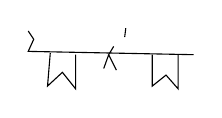
\begin{tikzpicture}[scale=.7]
\draw (0,.25)--(.1,.1)--(0,-.12)--(3,-.18);
\draw (.4,-.15)--(.35,-.75)--(.62,-.5)--(.86,-.8)--(.86,-.18);
\draw (2.25,-.18)--(2.25,-.75)--(2.5,-.55)--(2.72,-.8)--(2.72,-.18);
\draw (1.46,-.18)--(1.37,-.43) (1.46,-.18)--(1.6,-.46) (1.46,-.18)--(1.55,-.03);
\draw (1.75,.14)--(1.77,.3);
\end{tikzpicture}}

\deleted{\[
\boxed{G,\quad g_1,\qquad,\ g_r}
\]
\figure{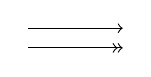
\begin{tikzpicture}\draw[->] (0,.25)--(1.2,.25);\draw[->>] (0,0)--(1.2,0);\end{tikzpicture}}
Diagramme de Cayley
\figure{\begin{tikzpicture}[scale=.9]
\coordinate (x) at (0,0);\coordinate (a) at (.1,1.2);\coordinate (b) at (1.65,1.18);
\draw (x)..controls (1.5,.8) and (4.4,1.1)..(3.9,2.1)..controls (3.3,3.2) and (.4,3.2)..(a);
\draw[->] (x)--(0.05,.62)--(a);\draw (x)..controls(-.1,.6)and(.05,.9)..(a);
\draw[->>] (a)--(.8,1.4);
\draw[->>] (x)--(.45,-.4);
\draw[->>] (x)--(.6,.38);\draw (.6,.38)--(b);
\fill (x) circle(1.6pt);\fill (a) circle(1.6pt);\fill (b) circle(1.4pt);
\node[below left] at(x){$x$};\node[below right] at(b){$xg_i$};
\fill (1.7,0) circle(1.1pt);\fill (3.4,0) circle(1.3pt);\fill (-1.6,.04) circle(1.1pt);\fill (-1.5,-.35) circle(1.1pt);
\draw (5.5,-.4)..controls(7.7,-.2)and(8.8,.2)..(8.3,1.4);
\node[below] at(5.5,-.4){$g$};\draw[->] (5.3,.15)..controls(5.3,-.1)..(5.5,-.25);
\end{tikzpicture}}
Mot \unsure{en les} $g_i$ $+$ origine
\[
g,\ g_i
\]}
\mspage{36}
